%\iffalse
\let\negmedspace\undefined
\let\negthickspace\undefined
\documentclass[journal,12pt,twocolumn]{IEEEtran}
\usepackage{cite}
\usepackage{amsmath,amssymb,amsfonts,amsthm}
\usepackage{algorithmic}
\usepackage{graphicx}
\usepackage{textcomp}
\usepackage{xcolor}
\usepackage{txfonts}
\usepackage{listings}
\usepackage{enumitem}
\usepackage{mathtools}
\usepackage{gensymb}
\usepackage{comment}
\usepackage[breaklinks=true]{hyperref}
\usepackage{tkz-euclide} 
\usepackage{listings}
\usepackage{gvv}                            \usepackage{tikz}
\usepackage{circuitikz}
\def\inputGnumericTable{}                                
\usepackage[latin1]{inputenc}                            
\usepackage{color}                                       
\usepackage{array}                                       
\usepackage{longtable}                                   
\usepackage{calc}                              
\usepackage{tikz}
\usepackage{multirow}                                    
\usepackage{hhline}                                      
\usepackage{ifthen}                            
\usepackage{caption}
\usepackage{lscape}
\usepackage{amsmath}
\newtheorem{theorem}{Theorem}[section]
\newtheorem{problem}{Problem}
\newtheorem{proposition}{Proposition}[section]
\newtheorem{lemma}{Lemma}[section]
\newtheorem{corollary}[theorem]{Corollary}
\newtheorem{example}{Example}[section]
\newtheorem{definition}[problem]{Definition}
\newcommand{\BEQA}{\begin{eqnarray}}
\newcommand{\EEQA}{\end{eqnarray}}
\newcommand{\define}{\stackrel{\triangle}{=}}
\theoremstyle{remark}
\newtheorem{rem}{Remark}

\begin{document}

\bibliographystyle{IEEEtran}
\vspace{3cm}

\title{GATE 2023 PH Q37}
\author{EE23BTECH11009 - AROSHISH PRADHAN$^{*}$% <-this % stops a space
}
\maketitle
\newpage
\bigskip
\textbf{Question:} An input voltage in the form of a square wave of frequency $1\, kHz$ is given to a circuit, which results in the output shown schematically below. Which one of the following options is the CORRECT representation of the circuit?

\begin{figure}[!h]
    \centering
    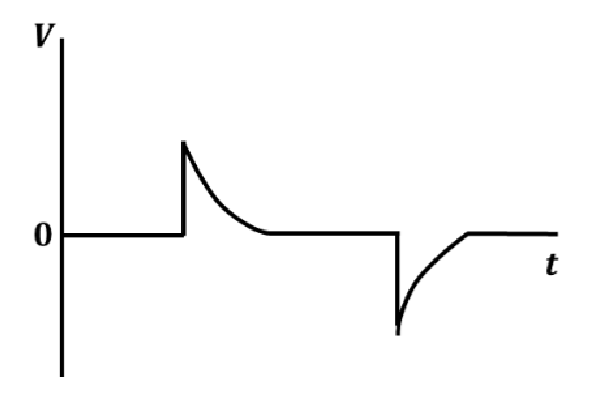
\includegraphics[width = \columnwidth]{figs/question.png}
    \caption{}
    \label{fig:ques_gate.ph.23.37}
\end{figure}

\begin{enumerate}[label = (\alph*)]
    \item
    \begin{minipage}[t]{\columnwidth}
        \begin{circuitikz}
    \draw(0, 0) to[short,*-*] ++ (4,0);
\draw (0,2) to[C,l=$0.1\mu F$, *-*] ++ (3,0) coordinate(a);
\draw (a) to[short,-*] ++ (1,0);
\draw (a) to[R, l_=$0.5k\Omega$,*-] ++(0,-2);

% Voltage labels
\draw (0,2) to[open,l_=V$_{in}$] ++(0,-2);
\draw (4,2) to[open,l=V$_{out}$] ++(0,-2);
\end{circuitikz}


    \end{minipage}
    \item
    \begin{minipage}[t]{\columnwidth}
        \begin{circuitikz}
    \draw(0, 0) to[short,*-*] ++ (4,0);
\draw (0,2) to[C,l=$1\mu F$, *-*] ++ (3,0) coordinate(a);
\draw (a) to[short,-*] ++ (1,0);
\draw (a) to[R, l_=$5k\Omega$,*-] ++(0,-2);

% Voltage labels
\draw (0,2) to[open,l_=V$_{in}$] ++(0,-2);
\draw (4,2) to[open,l=V$_{out}$] ++(0,-2);
\end{circuitikz}


    \end{minipage}
    \item
    \begin{minipage}[t]{\columnwidth}
        \begin{circuitikz}
    \draw(0, 0) to[short,*-*] ++ (4,0);
\draw (0,2) to[R, l = $0.5k\Omega$, *-] ++ (3,0) coordinate(a);
\draw (a) to[short,-*] ++ (1,0);
\draw (a) to[C,l_=$0.1\mu F$,*-*] ++(0,-2);

% Voltage labels
\draw (0,2) to[open,l_=V$_{in}$] ++(0,-2);
\draw (4,2) to[open,l=V$_{out}$] ++(0,-2);
\end{circuitikz}


    \end{minipage}
    \item
    \begin{minipage}[t]{\columnwidth}
        \begin{circuitikz}
    \draw(0, 0) to[short,*-*] ++ (4,0);
\draw (0,2) to[R, l = $5k\Omega$, *-] ++ (3,0) coordinate(a);
\draw (a) to[short,-*] ++ (1,0);
\draw (a) to[C,l_=$1\mu F$,*-*] ++(0,-2);

% Voltage labels
\draw (0,2) to[open,l_=V$_{in}$] ++(0,-2);
\draw (4,2) to[open,l=V$_{out}$] ++(0,-2);
\end{circuitikz}


    \end{minipage}
\end{enumerate}

\solution
\begin{table}[!h]
    \centering
    \begin{tabular}{|c|c|c|}
    \hline
       \textbf{Symbol}  & \textbf{Value} &  \textbf{Description}\\
    \hline
       $V_{in}$  &  &  Input Voltage\\
    \hline
        $V_{out}$ & & Output Voltage\\
    \hline
        $f$ & $1000Hz$ & Input Wave Frequency\\
    \hline
        $T$ & $\dfrac{1}{f} = 10^{-3} s$ & Input Wave Time Period\\
    \hline
        \multirow{4}{*}{$R$} & (a) $0.5k\Omega$ & \multirow{4}{*}{Resistance}\\
        \cline{2-2}
        & (b) $5k\Omega$ &\\
        \cline{2-2}
        & (c) $0.5k\Omega$ &\\
        \cline{2-2}
        & (d) $5k\Omega$ &\\
    \hline
        \multirow{4}{*}{$C$} & (a) $0.1\mu F$ & \multirow{4}{*}{Capacitance}\\
        \cline{2-2}
        & (b) $1\mu F$ &\\
        \cline{2-2}
        & (c) $0.1\mu F$ &\\
        \cline{2-2}
        & (d) $1\mu F$ &\\
    \hline
        $\tau$ & $RC$ & Time Constant\\
    \hline
    \end{tabular}
    \caption{Given Parameters}
    \label{tab:1_gate.23.ph.37}
\end{table}


Input waveform is a square wave (\figref{fig:square_gate.ph.23.37}), so we take its Fourier Transform 
\begin{align}
    V_{in}(t) &= 2\brak{2\sbrak{\frac{\brak{t-\frac{T}{4}}}{T}} - \sbrak{\frac{2\brak{t - \frac{T}{4}}}{T}}} + 1
\end{align}
Fourier Series Coefficient:
\begin{align}
    c_k = \frac{1}{T} \int_{T} V_{in}(t)e^{-jk\omega t}dt
\end{align}
As square wave is even, $\sin(k\omega t)$ terms become zero. Cosine coefficients are:
\begin{align}
    a_n &= \frac{2}{T} \int_{T} V_{in}(t) \cos\brak{\frac{2\pi nt}{T}}\\
    &= \frac{4}{n\pi}\sin{\brak{\frac{n\pi}{2}}}\cos\brak{{n\pi}}
\end{align}

Fourier Series of $V_{in}(t)$:
\begin{align}
    V_{in}(t) = \sum_{n = 1}^{\infty}a_n \cos\brak{\frac{2\pi nt}{T}}\label{eq:5_gate.23.ph.37}
\end{align}

\begin{figure}[!h]
    \centering
    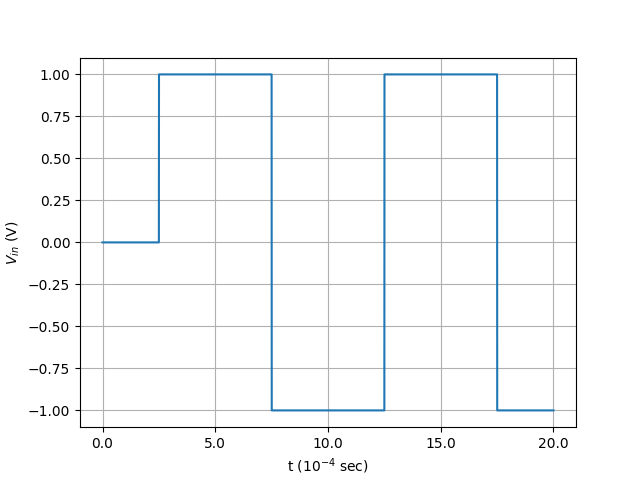
\includegraphics[width = \columnwidth]{figs/square.png}
    \caption{Input Square Waveform ($V_{in}(t)$)}
    \label{fig:square_gate.ph.23.37}
\end{figure}

Taking Fourier Transform of $V_{in}(t)$:
\begin{align}
    V_{in}(t) &\system{F} \mathcal{V}_{in}(j\omega)
\end{align}

\begin{figure}[!h]
    \centering
    \begin{circuitikz}
    \draw(0, 0) to[short,*-] ++ (3,0);
    \draw (0,2) to[C,l=$\frac{1}{sC}$, *-] ++ (3,0) coordinate(a);
    %\draw (a) to[short,-*] ++ (1,0);
    \draw (a) to[R, l_=$R$,*-] ++(0,-2);
    
    % Voltage labels
    \draw (0,2) to[open,l_=V$_{in}$] ++(0,-2);
    \end{circuitikz}
    \caption{Series RC Circuit in s-domain}
    \label{fig:s-domain_gate.ph.23.37}
\end{figure}

\begin{align}
    s &= j\omega\\
    \implies Z &= R + \frac{1}{sC}\\
    &= R + \frac{1}{j\omega C}
\end{align}

$\mathcal{V}_{in}(j\omega)$ was input into all four circuits and Inverse Fourier Transform was taken of the response.

Transfer Function:
\begin{align}
    H(j\omega) = \frac{V_{out}}{V_{in}}
\end{align}
\begin{enumerate}
    \item Option A
    \begin{align}
        H_R(j\omega) &=  \frac{R}{R + \frac{1}{j\omega C}}\\
        &= \frac{j\omega RC}{1+j\omega RC}\\
        &= \brak{\frac{\omega R C}{\sqrt{1 + (\omega R C)^2}}}e^{j\tan^{-1}\brak{\frac{1}{\omega RC}}}\label{eq:13_gate.23.ph.37}
    \end{align}
    \begin{figure}[!h]
        \centering
        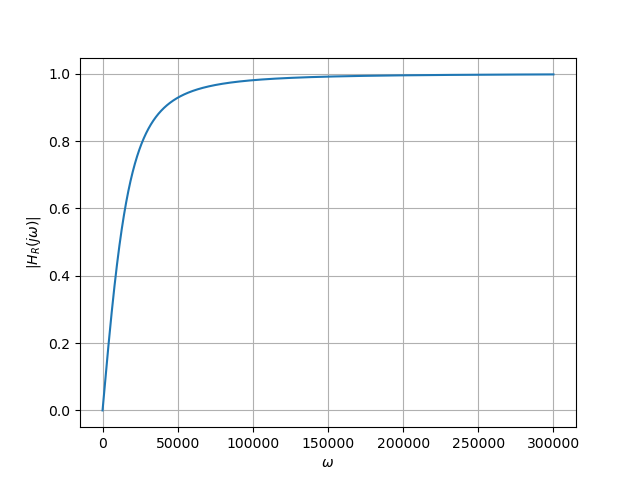
\includegraphics[width=\columnwidth]{figs/opt_a_hf.png}
        \caption{$\abs{H_R(j\omega)}$ vs $\omega$ for $R=0.5k\Omega$, $C=0.1\mu F$}
        \label{fig:opt_a_hf_gate.ph.23.37}
    \end{figure}
    \begin{align}
        \implies \mathcal{V}_{out}(j\omega) &= H_R(j\omega)\mathcal{V}_{in}(j\omega)\\
        \implies V_{out}(t) &= \mathcal{F}^{-1}\cbrak{H_R(j\omega)\mathcal{V}_{in}(j\omega)}\\
    \end{align}
    Using \eqref{eq:5_gate.23.ph.37} and \eqref{eq:13_gate.23.ph.37}, 
    \begin{multline}
    V_{out}(t)=\mathcal{F}^{-1}\brak{\frac{\omega R C e^{j\tan^{-1}\brak{\frac{1}{\omega RC}}}}{\sqrt{1 + (\omega R C)^2}}}\ast \\ \brak{\sum_{n = 1}^{\infty}\frac{4}{n\pi}\sin{\brak{\frac{n\pi}{2}}}\cos\brak{{n\pi}} \cos{\brak{n\omega t}}}
    \end{multline}
    \begin{figure}[!h]
        \centering
        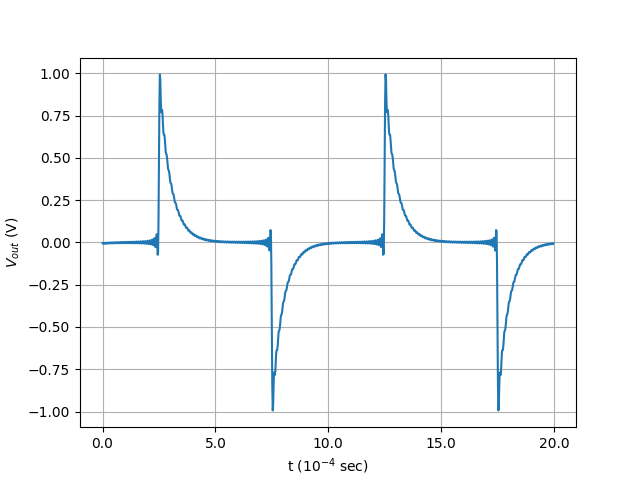
\includegraphics[width = \columnwidth]{figs/opt_a_res.png}
        \caption{Opt A: $V_{out}(t)$ vs $t$}
        \label{fig:opt_a_res_gate.23.ph.37}
    \end{figure}

    \item Option B
    \begin{align}
        H_R(j\omega) &=  \frac{R}{R + \frac{1}{j\omega C}}\\
        &= \frac{j\omega RC}{1+j\omega RC}\\
        &= \brak{\frac{\omega R C}{\sqrt{1 + (\omega R C)^2}}}e^{j\tan^{-1}\brak{\frac{1}{\omega RC}}}\label{eq:20_gate.23.ph.37}
    \end{align}
    \begin{figure}[!h]
        \centering
        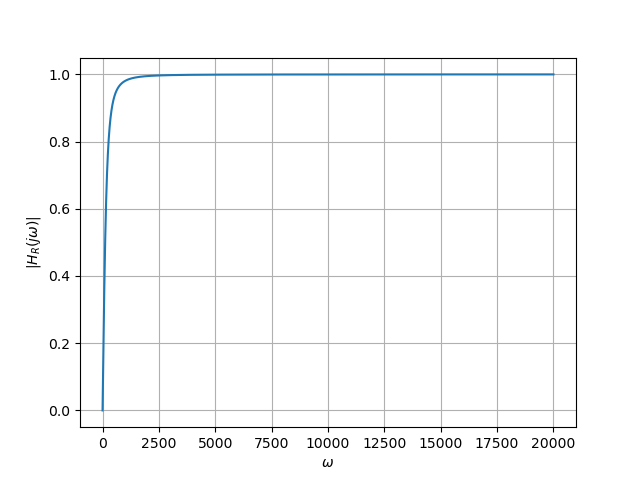
\includegraphics[width=\columnwidth]{figs/opt_b_hf.png}
        \caption{$\abs{H_R(j\omega)}$ vs $\omega$ for $R=5k\Omega$, $C=1\mu F$}
        \label{fig:opt_b_hf_gate.ph.23.37}
    \end{figure}
    \begin{align}
        \implies \mathcal{V}_{out}(j\omega) &= H_R(j\omega)\mathcal{V}_{in}(j\omega)\\
        \implies V_{out}(t) &= \mathcal{F}^{-1}\cbrak{H_R(j\omega)\mathcal{V}_{in}(j\omega)}
    \end{align}
     Using \eqref{eq:5_gate.23.ph.37} and \eqref{eq:20_gate.23.ph.37}, 
    \begin{multline}
    V_{out}(t)=\mathcal{F}^{-1}\brak{\frac{\omega R C e^{j\tan^{-1}\brak{\frac{1}{\omega RC}}}}{\sqrt{1 + (\omega R C)^2}}}\ast\\ \brak{\sum_{n = 1}^{\infty}\frac{4}{n\pi}\sin{\brak{\frac{n\pi}{2}}}\cos\brak{{n\pi}} \cos{\brak{n\omega t}}}
    \end{multline}
    \begin{figure}[!h]
        \centering
        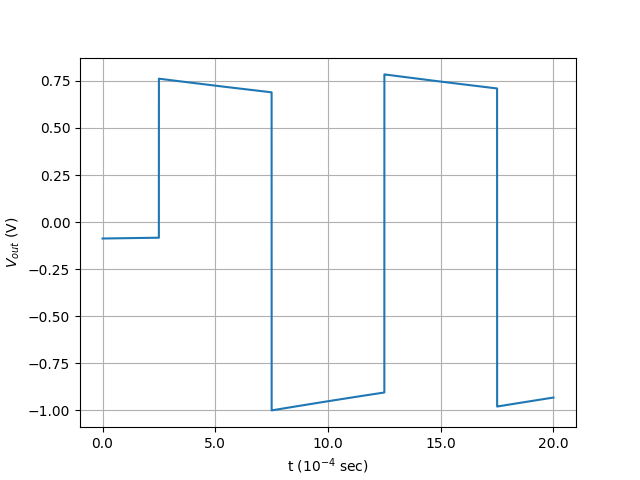
\includegraphics[width = \columnwidth]{figs/opt_b_res.png}
        \caption{Opt B: $V_{out}(t)$ vs $t$}
        \label{fig:opt_b_res_gate.23.ph.37}
    \end{figure}
    \newpage
    \item Option C
    \begin{align}
        H_C(j\omega) &=  \frac{\frac{1}{j\omega C}}{R + \frac{1}{j\omega C}}\\
        &= \frac{1}{1+j\omega RC}\\
        &= \brak{\frac{1}{\sqrt{1 + (\omega R C)^2}}}e^{-j\tan^{-1}\brak{\omega RC}}\label{eq:26_gate.23.ph.37}
    \end{align}
    \begin{figure}[!h]
        \centering
        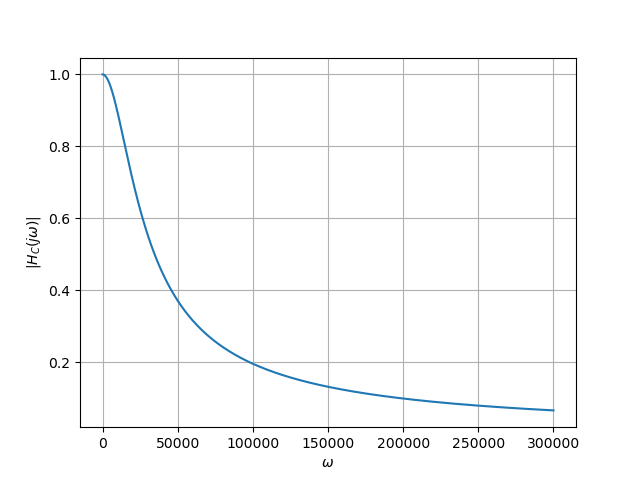
\includegraphics[width=\columnwidth]{figs/opt_c_hf.png}
        \caption{$\abs{H_C(j\omega)}$ vs $\omega$ for $R=0.5k\Omega$, $C=0.1\mu F$}
        \label{fig:opt_c_hf_gate.ph.23.37}
    \end{figure}
    \begin{align}
        \implies \mathcal{V}_{out}(j\omega) &= H_C(j\omega)\mathcal{V}_{in}(j\omega)\\
        \implies V_{out}(t) &= \mathcal{F}^{-1}\cbrak{H_C(j\omega)\mathcal{V}_{in}(j\omega)}
    \end{align}
     Using \eqref{eq:5_gate.23.ph.37} and \eqref{eq:26_gate.23.ph.37}, 
    \begin{multline}
    V_{out}(t)=\mathcal{F}^{-1}\brak{\frac{e^{j\tan^{-1}\brak{\frac{1}{\omega RC}}}}{\sqrt{1 + (\omega R C)^2}}}\ast\\ \brak{\sum_{n = 1}^{\infty}\frac{4}{n\pi}\sin{\brak{\frac{n\pi}{2}}}\cos\brak{{n\pi}} \cos{\brak{n\omega t}}}
    \end{multline}
    \begin{figure}[!h]
        \centering
        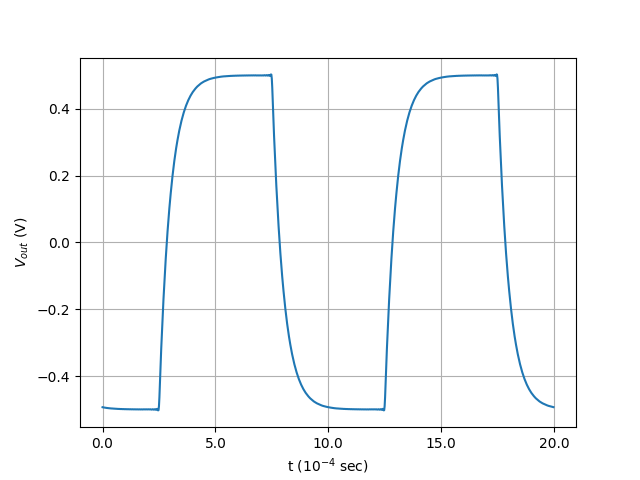
\includegraphics[width = \columnwidth]{figs/opt_c_res.png}
        \caption{Opt C: $V_{out}(t)$ vs $t$}
        \label{fig:opt_c_res_gate.23.ph.37}
    \end{figure}
    
    \item Option D
    \begin{align}
        H_C(j\omega) &=  \frac{\frac{1}{j\omega C}}{R + \frac{1}{j\omega C}}\\
        &= \frac{1}{1+j\omega RC}\\
        &= \brak{\frac{1}{\sqrt{1 + (\omega R C)^2}}}e^{-j\tan^{-1}\brak{\omega RC}}\label{eq:32_gate.23.ph.37}
    \end{align}
    \begin{figure}[!h]
        \centering
        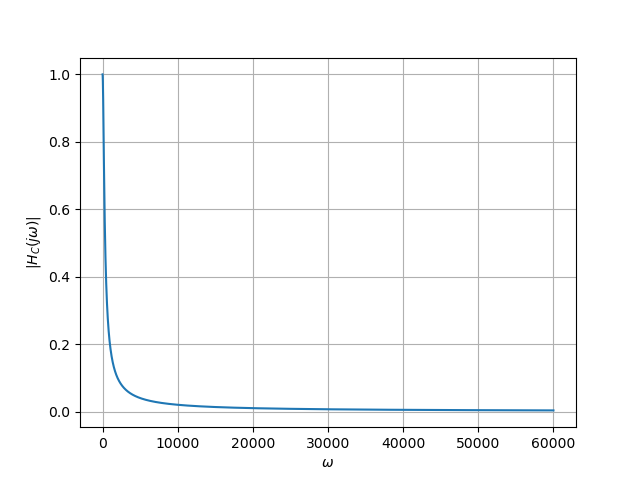
\includegraphics[width=\columnwidth]{figs/opt_d_hf.png}
        \caption{$\abs{H_C(j\omega)}$ vs $\omega$ for $R=5k\Omega$, $C=1\mu F$}
        \label{fig:opt_d_hf_gate.ph.23.37}
    \end{figure}
    \newpage
    \begin{align}
        \implies \mathcal{V}_{out}(j\omega) &= H_C(j\omega)\mathcal{V}_{in}(j\omega)\\
        \implies V_{out}(t) &= \mathcal{F}^{-1}\cbrak{H_C(j\omega)\mathcal{V}_{in}(j\omega)}
    \end{align}
    Using \eqref{eq:5_gate.23.ph.37} and \eqref{eq:32_gate.23.ph.37}, 
    \begin{multline}
    V_{out}(t)=\mathcal{F}^{-1}\brak{\frac{e^{j\tan^{-1}\brak{\frac{1}{\omega RC}}}}{\sqrt{1 + (\omega R C)^2}}}\ast\\ \brak{\sum_{n = 1}^{\infty}\frac{4}{n\pi}\sin{\brak{\frac{n\pi}{2}}}\cos\brak{{n\pi}} \cos{\brak{n\omega t}}}
    \end{multline}
    \begin{figure}[!h]
        \centering
        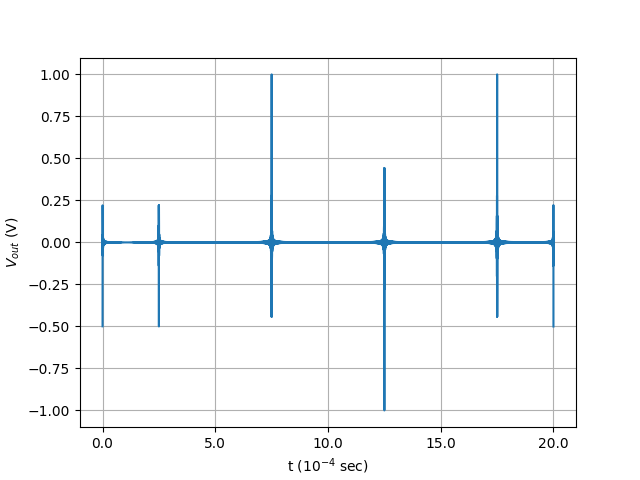
\includegraphics[width = \columnwidth]{figs/opt_d_res.png}
        \caption{Opt D: $V_{out}(t)$ vs $t$}
        \label{fig:opt_d_res_gate.23.ph.37}
    \end{figure}
\end{enumerate}
\end{document}

